%        File: lecture.tex
%     Created: Tue Sep 06 01:00 PM 2011 C
% Last Change: Tue Sep 06 01:00 PM 2011 C
%
\documentclass[letterpaper]{article}
\usepackage[acronym,toc]{glossaries}
\makeglossaries
\usepackage[top=1.0in,bottom=1.0in,left=1.0in,right=1.0in]{geometry}
\usepackage{verbatim}
\usepackage{amssymb}
\usepackage{graphicx}
\usepackage{longtable}
\usepackage{amsfonts}
\usepackage{amsmath}
\usepackage[usenames]{color}
\usepackage[
naturalnames = true, colorlinks = true, linkcolor = Black,
anchorcolor = Black,
citecolor = Black,
menucolor = Black,
urlcolor = Blue
]{hyperref}

\DeclareMathOperator{\erfc}{erfc}
\author{K. Huff
\\ \href{mailto:khuff@cae.wisc.edu}{\texttt{khuff@cae.wisc.edu}}
}
\date{}
\title{Development of a Performance Assessment Model:\\
Lecture Notes}
\begin{document}
\maketitle
\setcounter{tocdepth}{2}
\tableofcontents
\newacronym{MIT}{MIT}{the Massachusettes Institute of Technology}
\newacronym{UW}{UW}{University of Wisconsin}
\newacronym{US}{US}{United States}
\newacronym{SNF}{SNF}{spent nuclear fuel}
\newacronym{FEHM}{FEHM}{Finite Element Heat and Mass Transfer}
\newacronym{DOE}{DOE}{Department of Energy}
\newacronym{GENIUSv2}{GENIUS}{Global Evaluation of Nuclear Infrastructure Utilization Scenarios, Version 2}
\newacronym{CNERG}{CNERG}{Computational Nuclear Engineering Research Group}
\newacronym{GDSM}{GDSM}{Generic Disposal System Model}
\newacronym{GPAM}{GPAM}{Generic Performance Asessment Model}
\newacronym{FEPs}{FEPs}{Features, Events, and Processes}
\newacronym{EBS}{EBS}{Engineered Barrier System}
\newacronym{EDZ}{EDZ}{Excavation Disturbed Zone}
\newacronym{YMR}{YMR}{Yucca Mountain Repository Site}
\newacronym{EPA}{EPA}{Environmental Protection Agency}
\newacronym{PEI}{PEI}{Peak Environmental Impact}
\newacronym{VISION}{VISION}{the Verifiable Fuel Cycle Simulation Model}
\newacronym{NUWASTE}{NUWASTE}{Nuclear Waste Assessment System for Technical Evaluation}
\newacronym{NWTRB}{NWTRB}{Nuclear Waste Technical Review Board}
\newacronym{OCRWM}{OCRWM}{Office of Civillian Radioactive Waste Management}
\newacronym{UFD}{UFD}{Used Fuel Disposition}
\newacronym{DYMOND}{DYMOND}{Dynamic Model of Nuclear Development }
\newacronym{DANESS}{DANESS}{Dynamic Analysis of Nuclear Energy System Strategies}
\newacronym{CAFCA}{CAFCA}{ Code for Advanced Fuel Cycles Assessment }
\newacronym{ORION}{ORION}{O..}
\newacronym{NFCSim}{NFCSim}{Nuclear Fuel Cycle Simulator}
\newacronym{COSI}{COSI}{Commelini-Sicard}
\newacronym{FCT}{FCT}{Fuel Cycle Technology}
\newacronym{SWF}{SWF}{Separations and Waste Forms}
\newacronym{FCO}{FCO}{Fuel Cycle Options}
\newacronym{RDD}{RD\&D}{Research Development and Design}
\newacronym{WIPP}{WIPP}{Waste Isolation Pilot Plant}
\newacronym{ANDRA}{ANDRA}{Agence Nationale pour la gestion des D\'echets RAdioactifs, the French National Agency for Radioactive Waste Management}
\newacronym{TSM}{TSM}{Total System Model}
\newacronym{LANL}{LANL}{Los Alamos National Laboratory}
\newacronym{INL}{INL}{Idaho National Laboratory}
\newacronym{ANL}{ANL}{Argonne National Laboratory}
\newacronym{SNL}{SNL}{Sandia National Laboratory}
\newacronym{LBNL}{LBNL}{Lawrence Berkeley National Laboratory}
\newacronym{LLNL}{LLNL}{Lawrence Livermore National Laboratory}
\newacronym{NAGRA}{NAGRA}{National Cooperative for the Disposal of Radioactive Waste}
\newacronym{CUBIT}{CUBIT}{CUBIT Geometry and Mesh Generation Toolkit}
\newacronym{CSNF}{CSNF}{Commercial Spent Nuclear Fuel}
\newacronym{DSNF}{DSNF}{DOE Spent Nuclear Fuel}
\newacronym{HTGR}{HTGR}{High Temperature Gas Reactor}
\newacronym{TRISO}{TRISO}{Tristructural Isotropic}
\newacronym{MA}{MA}{Minor Actinide}
\newacronym{CEA}{CEA}{Commissariat a l'Energie Atomique et aux Energies Alternatives}
\newacronym{SKB}{SKB}{Svensk Karnbranslehantering AB}
\newacronym{SINDAG}{SINDA{\textbackslash}G}{Systems Improved Numerical Differencing Analyzer $\backslash$ Gaski}
%\newacronym{<++>}{<++>}{<++>}

\clearpage
\section{Groundwater Hydrology
\cite{schwartz_fundamentals_2003, wang_introduction_1982}}

Groundwater hydrology is the study of groundwater movement.

\subsection{Hydraulic Head }

Hydraulic head is the hydrologic indicator of potential energy. It has units of 
length, specifically height above a geological \emph{datum}, the zero point 
relative to which heads are measured. 

One way to derive this notion is according to Hubbart's derivation 
\cite{wang_introduction_1982}. The work to raise the water to a pressure, $P$, 
and the work required to raise the water to an elevation, $z$, are additive.

The work required to raise a mass, $m$, to a pressure, $P$, is described by the 
integral
\begin{align}
  W_P &= \frac{1}{m}\int_0^PVdP
  \intertext{where}
  m  &= \mbox{ mass of the water }[kg]\nonumber\\
  V  &= \mbox{ volume of the water }[m^3]\nonumber\\
  P  &= \mbox{ pressure }[ kg/m/s^2].\nonumber
\end{align}

In an incompressible fluid such as water, the work $W_P$ required to raise a 
unit mass
to some pressure, $P$, becomes
\begin{align}
  W_P &= P/\rho_w \label{workp}
  \intertext{where}
  \rho_w  &= \mbox{ the density of water}[kg/m^3].\nonumber
\end{align}

The work required to raise a unit mass to elevation $z$ from elevation $z_{ref}$  
(the `datum') is simply the work, $W_g$ against gravity
\begin{align}
  W_g &= g(z-z_{ref})
  \label{workg}
  \intertext{where}
  g  &= \mbox{ acceleration of gravity }[m/s^2].\nonumber
\end{align}

From these expressions for work the potential energy function, $\phi$, of the 
two  separate potentials, pressure and elevation, act additively on a unit mass 
of groundwater. Their combined effects can be written as the sum,
\begin{align}
  \phi &= W_P + W_g\nonumber\\
       &= \frac{P}{\rho_w} + g(z-z_{ref}.)
  \label{potentialfunc}
  \intertext{If}
  z_{ref} &= 0\nonumber
  \intertext{and the potential energy is directly proportional to gravity}
  \phi &= gh \nonumber
  \intertext{where}
  h &= \mbox{ Darcy's experimental head }[m],\nonumber
  \intertext{then}
  h &= \frac{\phi}{g}\nonumber\\
    &= \frac{P}{\rho_wg} + z\nonumber\\
    &=  \psi + z \label{bernoulli}
  \intertext{where}
  z &= \mbox{ elevation head }[m]\nonumber\\
  \psi &= \mbox{ pressure head }[m].\nonumber
\end{align}

Thus, the total hydraulic head, $h$, of a column of water is the vertical 
distance from the datum ($h=0$) to the height of the water surface.  Elevation 
head, $z$, is the distance from the datum to the measuring point in the flow 
field. The pressure head, $\psi$, is the pressure, $P$ in $[Pa]$, at that 
measurement point, divided by the density of the fluid, $\rho_w$, and the 
accelation of gravity, $g$. Pressure head, elevation head, and total head are 
shown in Figure
\ref{fig:head}. 

\begin{figure}[htbp!]
  \begin{center}
    \def\svgwidth{.7\textwidth}
    \input{head.eps_tex}
    \caption{Various types of head value in a column of water in a well are 
    measured with respect to the datum.}
    \label{fig:head}
  \end{center}
\end{figure}


Different lithologies and candidate sites have different head gradients. Due to 
anisotropies in their hydraulic conductivity tensors (see section 
\ref{subsec:cond}), some lithologies, such as clay, are less likely to have 
strong head gradients. 

\subsection{Porosity}

Porosity is a hydraulic parameter which significantly contributes to the 
hydraulic conductivity of a medium. 

The porosity of a medium is the ration of void volume, $V_v$, in the medium to 
the total volume, $V_T$ of the medium. As shown in Figure \ref{fig:wetDry}, the 
volume of water sufficient to saturate a packed sand matrix is equivalent to the 
void volume.

\begin{figure}[htbp!]
  \begin{center}
    \def\svgwidth{\textwidth}
    \input{wetDry.eps_tex}
  \end{center}
  \caption{The ratio of the volume of saturation water to the total packed sand 
  volume gives the porosity, $n$, in $[\%]$ \cite{heath_basic_1983}. }
  \label{fig:wetDry}
\end{figure}

The porosity of a material is therefore mathematically defined as \begin{align}
  n_T &= \frac{\mbox{void volume}}{\mbox{total volume}}\nonumber\\
      &= \frac{V_v}{V_T}\nonumber\\
      &= \frac{V_T-V_s}{V_T}
  \label{porosity}
  \intertext{where}
  n_T &= \mbox{ total porosity }[\%]\nonumber\\
  V_v &= \mbox{ void volume }[m^3]\nonumber\\
  V_T &= \mbox{ total volume }[m^3]\nonumber\\
  V_s &= \mbox{ volume of solids }[m^3].\nonumber
  \intertext{The dry solid volume can be defined as}
  V_s    &= \frac{m_s}{\rho_s}
  \intertext{and the total dry volume can be defined as}
  V_T    &= \frac{m_s}{\rho_b},
  \intertext{where}
  \rho_s &= \mbox{ grain density, or density of solids }[kg/m^3]\nonumber\\
  m_s    &= \mbox{ mass of solids }[kg]\nonumber\\
  \intertext{and}
  \rho_b &= \mbox{ bulk (dry) density }[kg/m^3],\nonumber\\
  \intertext{equation \eqref{porosity} can be rewritten}
  n_T    &= 1 - \frac{\rho_b}{\rho_s}.
\end{align}

The total porosity is a combination of primary and secondary porosity, shown in 
Figure \ref{fig:porosity}. Primary porosity is the macroscopically homogeneous  
void space present between grains in a geological matrix. This type of porosity 
includes empty space between grains of sand or consolidated rock characteristic 
of the level of packing or method of consolidation of the matrix. Secondary 
porosity is not intrinsic
to the rock, but induced in it. Examples of secondary porosity include features  
such as fractures, lava tubes, and caverns.

\begin{figure}[htbp!]
  \begin{center}
    \def\svgwidth{.8\textwidth}
    \input{porosity.eps_tex}
  \end{center}
  \caption{Primary porosity, a homogeneous characteristic of the rock matrix, 
  and secondary porosity, such as discrete fractures, caverns, and lava tubes,
  both contribute to total porosity \cite{heath_basic_1983}.} 
  \label{fig:porosity}
\end{figure}

Equipped with a notion of the total porosity, it is possible to define the 
effective porosity shown in figure \ref{fig:effPorosity}, which is the 
interconnected porosity through which fluid may flow, \begin{align}
  n_{eff} &= \frac{V_c}{V_T}n_T.  \label{effPorosity}
  \intertext{where}
  V_c &= \mbox{ interconnected volume. }\nonumber
\end{align}
Effective porosity is more influential on ground water flow in a porous medium 
than the total porosity, as it contributes to the permeability of the medium.  
In some media, the effective porosity is significantly different than the total  
porosity, resulting in much lower flow rates than the total porosity alone would 
indicate. Granite, for example, has an effective porosity that is nearly three 
magnitudes lower than its total porosity. 

\vspace{1cm}
\begin{figure}[htbp!]
  \begin{center}
    \def\svgwidth{.5\textwidth}
    \input{effPorosity.eps_tex}
  \end{center}
  \caption{A medium with a poorly connected pore volume has low effective 
  porosity, and vice versa.}
  \label{fig:effPorosity}
\end{figure}

\subsection{Darcy's Law}

Darcy's Law is analgous to Fourier's Law of heat conduction, and states that 
flow occurs as a function of a head gradient with a speed that obeys the 
hydraulic properties of the medium. Darcy's law for one dimensional flow is 

\begin{align}
  \frac{Q}{A} &= -K\frac{h_2 - h_1}{l_2-l_1} \label{darcy1d}
  \intertext{where}
  Q &= \mbox{ volumetric flow rate }[m^3/s]\nonumber
  \intertext{and}
  A &= \mbox{ cross sectional area of flow field }[m^2]\nonumber\\
  K &= \mbox{ hydraulic conductivity }[ m/s ].\nonumber\\
  h_i &= \mbox{ hydraulic head measured at point i } [m]\nonumber\\
  l_i &= \mbox{ linear position of point i } [m]\nonumber
\end{align}

Using the the definition of specific discharge (also known as Darcy flux), $q = 
Q/A$, and expressing the law in its differential form gives

\begin{align}
  q &= -K\frac{\partial h}{\partial l}.
  \label{darcy1ddiff}
\end{align}
  
The three dimensional form requires that the one dimensional form in equation 
\eqref{darcy1ddiff} be true for each spatial component, such that

\begin{align}
  \vec{q} &= -K\nabla{h}
  \label{darcy3d}
  \intertext{where}
  \vec{q} &= \mbox{ specific discharge vector }[m^3/s]\nonumber\\
  &= q_x\hat{\imath} + q_y\hat{\jmath} + q_z\hat{k}\nonumber
  \intertext{and}
  \nabla{h} &= \frac{\partial h}{\partial x} + \frac{\partial h}{\partial y} + 
  \frac{\partial h}{\partial z}. \nonumber
\end{align}

In the case of anisotropic media, the hydraulic conductivity, $K$ is given as a 
spatially heterogenous tensor, $\textbf{K}$. The general, three dimensional, 
anisotropic Darcy equation is therefore 

\begin{align}
  \vec{q} &= -\textbf{K}\nabla{h}
  \label{darcyanisotropic}
  \intertext{where}
  \textbf{K} &= \mbox{ hydraulic conductivity tensor }[ m/s ].\nonumber
\end{align}

\subsection{Hydraulic Conductivity}
\label{subsec:cond}

The hydraulic conductivity of a medium is a tensor that describes the ease with 
which water passes through the pore spaces of the medium in all directions.  
This tensor may be homogeneous or heterogeneous and isotropic or anisotropic. 

\subsubsection{Heterogeneity of the Hydraulic Conductivity}

Heterogeneity of a hydrogeological unit describes the spatial variability of the 
hydraulic conductivity. If the hydraulic conductivity is the same when
measured at all points in the hydrogeological medium,

\begin{align}
  \forall i,j \in V : K(x_i,y_i,z_i) = K(x_j,y_j,z_j),
  \label{homogeneous}
\end{align}
then the medium is homogenous. If instead, the hydraulic conductivity is
different at different locations, such that 
\begin{align}
  \exists i\ne j \in V : K(x_i,y_i,z_i) \ne K(x_j,y_j,z_j),
  \label{heteroeneous}
\end{align}

then the medium is heterogeneous.

\subsubsection{Anisotropy of the Hydraulic Conductivity}

Anisotropy of a hydrogeological unit describes the local directional dependence 
of the hydraulic conductivity tensor. Specifically, at a single location, an 
isotropic medium will demonstrate the same hydraulic conductivity in all 
directions, while an anisotropic medium will not.

Mathematically speaking, if the conductivity is constant at all measurement 
angles, $\theta$, such that

\begin{align}
  \forall \theta_i,\theta_j \in (0,2\pi) : K(\theta_i,x,y,z) = K(\theta_j,x,y,z) 
  \\
  \label{isotropic}
\end{align}
then the medium is isotropic. If instead, the angular components of the
hydraulic conductivity are nonconstant, such that
\begin{align}
  \exists \theta_i\ne\theta_j \in (0,2\pi) : K(\theta_i,x,y,z) \ne 
  K(\theta_j,x,y,z),
  \label{anisotropic}
\end{align}
then the medium is anisotropic and the tensor is expressed most generally,
\begin{align}
  \textbf{K} &= \mbox{ hydraulic conductivity tensor }[ m/s ]\nonumber\\
             &= \left[ \begin{array}{ccc}
                K_{xx}  & K_{xy}  & K_{xz}  \\
                K_{yx}  & K_{yy}  & K_{yz}  \\
                K_{zx}  & K_{zy}  & K_{zz}  \end{array} \right]
    \label{condfull}
    \intertext{where}
    K_{ij} &=\mbox{jth component in the i direction}.\nonumber
\end{align}
The general tensor in equation \eqref{condfull} is a second rank symmetric 
tensor and can always be simplified by aligning the tensor with the principal 
axis of anisotropy\cite{schwartz_fundamentals_2003}. This principal direction is 
defined by the directions of maximum ($K_{\parallel}$), minimum ($K_{\perp}$), 
and intermediate ($K_{\parallel}\times K_{\perp}$) hydraulic conductivity. That 
is, by aligning the tensor with the flow axis, it may be reduced to a diagonal 
matrix,

\begin{align}
    \textbf{K} &= \left[ \begin{array}{ccc}
                 K_{xx}  & 0       & 0  \\
                 0       & K_{yy}  & 0  \\
                 0       & 0       & K_{zz}  \end{array} \right].
  \label{conddiag}
\end{align}


\section{Mechanisms of Solute Transport}

Solutes in groundwater are transported due to various mechanisms.

\subsection{Diffusion}
\label{ss:diffusion}

Solutes will move from a location of high concentration to a location of low 
concentration due to the random thermal kinetic enery of the solute. Brownian 
motion is responsible for diffusion.

\begin{figure}[htbp!]
  \begin{center}
    \def\svgwidth{.6\textwidth}
    \input{Diffusion.eps_tex}
  \end{center}
  \caption{In diffusive transport, particles move according to random thermal 
  motion down the concentration gradient \cite{jrpol_diffusion.svg_2011}.}
  \label{fig:Diffusion}
\end{figure}

A mathematical description of this phenomenon can be addressed by describing the 
particle's motion as a random walk and applying statistical analysis. Another 
derivation of this phenomenon describes the flux, $J$ through a plane in a 
volume, and gives Fick's Law for porous media,

\begin{align}
  J_{xdif} &= -D' \frac{dC}{dx}\nonumber\\
  \label{ficks}
  \intertext{where}
  J_x &= \mbox{ Mass flux through the y-z plane }[kg/m^2/s]\nonumber\\
  D' &= \mbox{ Effective diffusion coefficient }[m^2/s]\nonumber\\
  C &= \mbox{ Concentration }[kg/m^3].\nonumber\\
\end{align}

The determination of the diffusion coefficient can be empirical or analytical.  
The Arrhenius equation gives a thermal dependence of the diffusion coefficient 
as does the Stokes-Einstein relationship.

The effecive diffusion coefficient for porous media is dependent on porosity and  
tortuosity, which affect the diffusion behavior of a solute. In a saturated porous 
medium, diffusion takes place only within the pore volume where liquid is 
present. To take this into account, the effective diffusion coefficient in a 
porous medium is reduced by both the absence of fluid in the matrix volume, and 
by the so-called ``tortuosity'' of the pathways. 

\begin{align}
  J_{xdif} &= -n\tau D_m \frac{dC}{dx}\\
  \label{ficks}
  \intertext{where}
  J_{xdif} &= \mbox{ Mass flux through the y-z plane in a porous medium}[kg/m^2/s]\nonumber\\
  n &= \mbox{ porosity }[\%]\nonumber\\
  \tau &= \mbox{ tortuosity }[-]\nonumber\\
  D_m &= \mbox{ Molecular diffusion coefficient }[m^2/s]\nonumber\\
  C &= \mbox{ Concentration }[kg/m^3].\nonumber
\end{align}

The tortuosity of a saturated porous medium can be estimated from the porosity 
with an equation developed by Millington and Quirk (1961),

\begin{align}
  \tau &= \frac{n_w^{7/3}}{n^2} \label{millington}
  \intertext{which for a saturated medium is estimated as }
  \tau &= n^{1/3}.  \\
  % Below is true, but where to put it . . . ?
  % D' = n\tau D_m = nD^{\star}
\end{align}


\subsection{Dispersion \cite{schwartz_fundamentals_2003}}

Solutes can be driven to move due to mechanical mixing, known as dispersion.  
Solutes acting under dispersion may travel further than they would due to 
advection alone. During fluid mixing in which a fluid with one solute 
concentration displaces a fluid with another concentration, dispersion causes a 
zone of mixing to develop around the advective front.

Dispersion in groundwater is caused by a combination of two phenomena. The first 
is mechanical dispersion, in which local variability of the fluid velocity 
around the mean due to mechanical heterogeneities of the rock at many scales.  
The second phenomenon is diffusion, discussed in section \ref{ss:diffusion}.

A mathematical description of this phenomenon will come generally from fluid 
dynamics. The total mechanical dispersive and diffusive phenomena can be 
combined as a total dispersive expression,
\begin{align}
  D &= D_{mdis} + \tau D_m
  \intertext{where}
  D_{mdis}&= \mbox{ coefficient of mechanical dispersivity }[m^2/s]\nonumber\\
          &=\alpha_{L} \frac{v_x^2}{|v|} + \alpha_{TH} \frac{v_y^2}{|v|} + 
          \alpha_{TV} \frac{v_z^2}{|v|},\\ \alpha_L  &= \mbox{ longitudinal 
          dispersivity }[m],\nonumber\\
  \alpha_{TH}  &= \mbox{ horizontal transverse dispersivity }[m],\nonumber\\
  \alpha_{TV}  &= \mbox{ vertical transverse dispersivity }[m],\nonumber\\
  \tau &= \mbox{ tortuosity }[-],\nonumber
  \intertext{and}
  D_m &= \mbox{ coefficient of molecular diffusion }[m^2/s]\nonumber.
  \label{totaldisp}
\end{align}
The dispersive mass flux can therefore be described, as in Burnett and Frind, 
1987,
\begin{align}
  J_{dis} &= J_{mdis} + J_{dif} \\
          &= -n\left(D_{mdis} + \tau D_m\right)\nabla C\\
          &= -nD\nabla C
  \label{dispflux}
  \intertext{where}
  D &= \left[ \begin{array}{ccc}
                D_{xx}  & D_{xy}  & D_{xz}  \\
                D_{yx}  & D_{yy}  & D_{yz}  \\
                D_{zx}  & D_{zy}  & D_{zz}  \end{array} \right],\nonumber\\
  D_{ij} &=
         \begin{cases} \alpha_{L} \frac{v_x^2}{|v|} + \alpha_{TH} 
           \frac{v_y^2}{|v|} + \alpha_{TV} \frac{v_z^2}{|v|} &  i=j=x,\\
                       \alpha_{L} \frac{v_y^2}{|v|} + \alpha_{TH} 
                       \frac{v_x^2}{|v|} + \alpha_{TV} \frac{v_z^2}{|v|} 
                       + \tau  D_m & i=j=y,\\
                       \alpha_{L} \frac{v_z^2}{|v|} + \alpha_{TV} 
                       \frac{v_y^2}{|v|} + \alpha_{TV} \frac{v_x^2}{|v|}  
                       + \tau D_m & i=j=z,\\
                       \left(\alpha_L - \alpha_{TH}\right)\frac{v_xv_y}{|v|} 
                       + \tau D_m & i=x, j=y,\\
                       \left(\alpha_L - \alpha_{TV}\right)\frac{v_xv_z}{|v|} & 
                       i=(x,z),j=(z,x),\\
                       \left(\alpha_L - \alpha_{TV}\right)\frac{v_yv_z}{|v|} & 
                       i=(y,z), j=(z,y),\\
         \end{cases}
\intertext{and}
|v| &= \sqrt{v_x^2 +v_y^2 + v_x^2}.
\end{align}
For uniform flow, where $v=v_x$ and $v_y=v_z=0$,
\begin{align}
  D_x &= D_L \nonumber\\
      &= \alpha_L v_x + \tau D_m\\
  D_y &= D_{TH} \nonumber\\
      &= \alpha_{TH} v_x + \tau D_m\\
  D_z &= D_{TV} \nonumber\\
      &= \alpha_{TV} v_x + \tau D_m.
  \label{uniflow}
\end{align}

\subsection{Advection}

Solutes are transported by advection when they move along with the water in 
which they are dissolved. The expression for mass flux due to dispersion can be 
added to the expression for mass flux due to advection to give total mass flux 
due to both,

\begin{align}
  J &=  J_{mdis} + J_{dif} + J_{adv}\\
    &=  J_{dis} + J_{adv}\\
    &= -nD\nabla C + nvC\\
    &=\left(-nD_{xx} \frac{\partial C}{\partial x}
            -nD_{xy} \frac{\partial C}{\partial y}
            -nD_{xz} \frac{\partial C}{\partial z}
             + nv_xC \right)\hat{\imath} \nonumber\\
    & + \left(-nD_{yx} \frac{\partial C}{\partial x}
            -nD_{yy} \frac{\partial C}{\partial y}
            -nD_{yz} \frac{\partial C}{\partial z}
            + nv_yC \right)\hat{\jmath} \nonumber\\
    & + \left(-nD_{zx} \frac{\partial C}{\partial x}
            -nD_{zy} \frac{\partial C}{\partial y}
            -nD_{zz} \frac{\partial C}{\partial z}
            + nv_zC \right)\hat{k}.
            \label{jadvdisp}
\end{align}

For unidirectional flow

\begin{align}
  J &=\left(-nD_{xx} \frac{\partial C}{\partial x}
             + nv_xC \right)\hat{\imath}
             + \left( -nD_{yy} \frac{\partial C}{\partial y}
            \right)\hat{\jmath}
            + \left( -nD_{zz} \frac{\partial C}{\partial z}
            \right)\hat{k}.
            \label{jadvdisp}
\end{align}



\section{Geochemistry}

Geochemical phenomena significantly affect solute transport. As such, the 
geochemical attributes of various environments contribute differently to 
repository performance.

\subsection{Saturated and Unsaturated Environments}

Saturated repository concepts are found below the water table. Water permeates 
the rock.

Unsaturated repository concepts are found above or near the top of the water 
table. Water does not permeate the rock.

Current investigations are focused primarily on saturated environments.

\subsection{Reducing and Oxidizing Environments\cite{mason_oxidation_1949}}

Elements exist in various oxidation states, a positive or negative number  
refering to the charge of the atom due to the number of electrons it posesses.
Oxidation refers to the increase of the oxidation state number of an element, 
and reduction is the opposite.  That is, while oxidation is the chemical loss of 
electrons by an atom, reduction is the gaining of electrons by an atom. 

The redox potential is the tendency in potential energy for an element to give 
up its electron and become more oxidized. This  potential energy is measured 
relative to the potential for hydrogen atoms at unit concentration to lose 
electrons and become oxidized, in volts,
\begin{align}
  H_2 \rightarrow 2H^+  + 2e.
  \label{hydrogen}
\end{align}

The potential for the redox equation in equation \eqref{hydrogen} is chosen to 
be 0 volts, such that for positive values of the redox potential, reactions tend 
to proceed in the oxidation direction. Accordingly, reactions proceed in
the reduction direction for negative potentials.

Closed, saturated envrionments are reducing. Unsaturated environments and 
environments that are saturated and open are oxidizing. 

The far field of most reducing environments are slightly oxidizing as they reach 
the zone near the overlying aquifer.

\subsection{Salinity}

Salinity affects sorption and solubility behaviors. It also expedites corrosion.  
Finally, salt is an important indicator of the historical flow at a site.  Where 
should salinity information get incorporated in this model?

\subsection{Sorption}

Sorption is a factor that retards movement, in which solutes are incorporated 
into the surfaces of pores or fractures (adsorption) or incorporated into the 
rock matrix (absorption). More specificially, when water with some solute 
concentration, $C_i$, meets a porous medium or a granular solid, the reaction 
proceeds toward an equilibrium in which the solute mass has partitioned between 
the solution and the solid, such that,
\begin{align}
  S&=\frac{V_w(C_i -C)}{m_s}
  \intertext{where}
  S &= \mbox{ mass sorbed on the surface }[kg/kg]\nonumber\\
  V_w &= \mbox{ volume of the solution  }[m^3]\nonumber\\
  C_i &= \mbox{ initial concentration in the solution }[kg_m^3]\nonumber\\
  C &= \mbox{ equilibrium concentration in the solution }[kg/m^3]\nonumber\\
  m_s &= \mbox{ sediment mass }[kg].\nonumber
\end{align}
The function $S(C)$ is called a sorption isotherm. Two common forms for the 
sorption isotherm are
\begin{align}
  S &= \begin{cases}
    \text{Freundlich : } & KC^n\\ \text{Langmuir : } &\frac{Q^0KC}{1+KC}\\ 
  \end{cases}
  \label{isotherms}
  \intertext{where}
  K &= \mbox{ partition coefficient }[m^3/kg]\nonumber\\
  n &= \mbox{ shaping constant }[-]\nonumber
  \intertext{and}
  Q^0 &= \mbox{ maximum sorptive capacity }[kg/kg].\nonumber
  \intertext{If in the Freundlich isotherm,}
  n &=1, \intertext{then}
  S &= K_dC
  \intertext{where}
  K_d &= \mbox{ the distribution coefficient }[m^3/kg],\nonumber
\end{align}
and the isotherm becomes very easy to incorporate into the mass transport 
equations, as in equation \eqref{linisomasstrans}.

The simplest way to model sorption is with a linear isotherm and tabulated 
values.  Sorption coefficients such as $K_d$ are tabulated elementally because 
the character of the equilibrium reaction is element specific. For example, 
iodine has different sorption behavior than carbon. These coefficients are
also host rock specific. That is, each element has different sorption behaviors 
in clay than in granite. 

Geochemistry also plays a role, and sorption for some elements are higher in
reducing environments. Sorption for some elements may be higher in oxidizing
environments. 

\subsection{Solubility} 

The dissolution behavior of solutes in aqueous solutions is called its 
solubility. This behavior is limited by the solute's solubility limit, described  
by an equilibrium constant that depends upon temperature, water chemistry, and 
the properties of the element. The solubility constant for ordinary solutes, 
$K_s$ gives units of concentration, $[kg/m^3]$,   and can be determined 
algebraically by the law of mass action which gives the partitioning at 
equilibrium between reactants and products.  For a reaction
\begin{align}
  cC + dD &= yY + zZ,
  \intertext{where}
  c,d,y,z  &= \mbox{ amount of respective constituent }[mol]\nonumber\\
  C,D  &= \mbox{ reactants }[-]\nonumber\\
  Y,Z  &= \mbox{ products }[-]\nonumber,
  \intertext{the law of mass action gives}
  K &= \frac{(Y)^y(Z)^z}{(C)^c(D)^d}
  \intertext{where}
  (X)  &= \mbox{ the equilibrium molal concentration of X }[mol/m^3]\nonumber\\
  K  &= \mbox{ the equilibrium constant }[-].\nonumber
  \label{massaction}
\end{align}
The equillibrium constant for many reactions are known, and can be found in 
chemical tables. Thereafter, the solubility constraints of a solution at 
equilibrium can be found algebraically.  In cases of salts that  dissociate in 
aqueous solutions, this equilibrium constant is called the salt's solubility 
product $K_{sp}$.

This equillibrium model, however, is only appropriate for dilute situations, and 
nondilute solutions at  partial equilibrium must be treated with an activity 
model by substituting the activities of the constituents  for their molal 
concentrations,
\begin{align}
  [X] &= \gamma_x(X)
  \intertext{where}
  [X]  &= \mbox{ activity of X }[-]\nonumber\\
  \gamma_x  &= \mbox{ activity coefficient of X}[-]\nonumber\\
  (X)  &= \mbox{ molal concentration of X}[mol/m^3]\nonumber
  \intertext{such that}
  IAP &= \mbox{ Ion Activity Product }[-].\nonumber\\
      &= \frac{[Y]^y[Z]^z}{[C]^c[D]^d}\\
  \label{IAP}
\end{align}
The ration between the IAP and the equillibrium constant $(IAP/K)$ quantifiesn
the departure from equilibrium of a solution.  This information is useful during 
the transient stage in which a solute is first introduced to a solution. When 
$IAP/K<1$, the solution is undersaturated with respect to the products. When, 
conversely, $IAP/K>1$, the solution is oversaturated and precipitation of solids 
in the volume will occur. 

Two models of mass balance applicable to a control volume incorporating 
solubility
limitation include the Ahn and Hedin models.

\subsubsection{Ahn Solubility Limited Release Model}

In the Ahn models, radionuclides with lower solubility coefficients are modeled 
with
the solubility limited release model.  Solubility values are assumed from TSPA
for this model, and elements with a solubility of less than $~5\times 10^{-2}
[mol/m^3]$ are taken to be
`low.' Elements in this `low' category include Zr, Nb, Sn and some toxic 
actinides such as Th and Ra for an oxidizing, unsaturated environment similar to 
the Yucca Mountain Repository.
It should be noted that in a reducing environment, the actinides are not as 
mobile, and the high and low solubility radionuclides will differ from this 
model.
This model suggests that dissolution of radionuclides into the flowthrough water 
is dominated by diffusion, which is largely dependent upon the concentration 
gradient between the waste matrix and the water. The mass balance driving 
radionuclide release takes the form:

\begin{equation}
 \dot{m_i}=8\epsilon D_eS_iL\sqrt{\frac{Ur_0}{\pi D_e}}
\end{equation} 

where $\epsilon$, U, $r_0$, and L are the geometric and
hydrologic factors porosity, water velocity, waste package radius, and waste
package length, respectively. $D_e$ is the effective diffusion coefficient
($m^2/yr$)  and $S_i$ is the solubility ($kg/m^3$) of isotope $i$.


\subsubsection{Hedin Solubility Limited Release Model}

In the Hedin model of the waste matrix, the amount of solute available within
the waste package is solved for, and for radionuclides with low solubility, the 
mass
fraction released from the waste matrix is limited by a simplified description
of their solubility. That is, 

\begin{align} m_{1i}(t)\le v_{1i}(t)C_{sol}
\end{align}

where the mass $m_{1i}$ in $[kg]$ of a radionuclide $i$ dissolved into the waste 
package
void volume $v_1$ in $[m^3]$, at a time t, is limited by the solubility limit, 
the maximum concentration, $C_{sol}$ in $[kg/m^3]$ at which that radionuclide is 
soluble \cite{hedin_integrated_2002}.

Various things affect solubility. Temperature, salinity, etc.

A good model for solubility limitation is at the release boundary of the volume, 
for mixed volumes.


\section{Solid Dissolution}

Dissolution occurs after some kind of alteration and degradation. 

Alteration is when some chemical reaction changes the characteristics  of a 
material. 

Give glass example. 

Show that there are physical dissolution models being generated. 

Waste form dissolution results may take place at a constant rate, a time 
dependent rate, or  a physical model dependent on both static and dynamic 
parameters such as temperature, water velocity, or pH. 

\subsection{Waste Package Failure}

Waste package failure is described best by a probability distribution such that 
a few packages can fail discretely at any one time. 


It's also possible that a good model would fail all of the waste packages 
fractionally at some rate. This will affect both the water going in and the 
water coming out, but it's not clear to me how much this will affect those 
things. 


\section{Solute Transport in Porous Media}

\subsection{Derivation \cite{van_genuchten_analytical_1982, 
leij_analytical_1991}}

Here we shall derive the general equation for solute transport in heterogeneous 
porous media.

As discussed in previous sections, mass transport by advection is driven by bulk 
water velocity, diffusion is the result of random thermal motion and tends  to 
drive solutes down concentration gradients, and hydraulic dispersion
results from heterogeneities in the water velocity field and drives accelerated 
mixing at the head of advection fronts.

Fundamentally, the effect of these phenomena on mass transport is captured by 
the conceptual mass conservation expression \begin{align}
  \mbox{In} - \mbox{Out} &= \mbox{Change in Storage}
  \label{inout}
\end{align} which describes the mass balance within a reference volume of porous 
media.

By rearranging equation \ref{inout} and defining incoming and outflowing fluxes 
in a control  volume,  solute transport in a permeable medium of homogeneous 
porosity can be
written (as in Schwartz and Zhang \cite{schwartz_fundamentals_2003})

\begin{align} \frac{\partial n C}{\partial t} & = - \nabla \cdot  (F_c + F_{dc} 
  + F_d) + m \label{solperm}
  \intertext{where} \displaybreak[0]
  n &= \mbox{solute accessible porosity } [\%]\nonumber\\
  C &= \mbox{ concentration } [kg \cdot m^{-3}]\nonumber\\ t &= \mbox{ time } 
  [s]\nonumber\\ F_c &= \mbox{ advective flow } [kg \cdot m^{-2}\cdot 
  s^{-1}]\nonumber\\
  &= nvC \nonumber \\
  \displaybreak[0]
  F_{dc} &= \mbox{ dispersive flow } [kg \cdot m^{-2}\cdot s^{-1}]\nonumber\\ &= 
  \alpha nv \nabla C  \nonumber\\ \displaybreak[0]
  F_d &= \mbox{ diffusive flow } [kg \cdot m^{-2}\cdot s^{-1}]\nonumber\\
  &= nD_e \nabla C\nonumber\\
  \displaybreak[0]
  m &= \mbox{ solute source } [kg \cdot m^{-3}\cdot s^{-1}].\nonumber
  \displaybreak[0]
  \intertext{In the expressions above,} v &= \mbox{ advective velocity } [m\cdot 
  s^{-1}] \nonumber\\
  \alpha &= \mbox{ dispersivity } [m]\nonumber\\
  D_e &= \mbox{ effective diffusion coefficient } [m^2\cdot s^{-1}]\nonumber
  \displaybreak[0]
  \intertext{and} n\cdot v &= \mbox{ Darcy flux } [m\cdot s^{-1}].
\end{align} 

The method by which the dominant solute transport mode (diffusive or advective)
is determined for a particular porous medium is by use of the dimensionless
Peclet number, 

\begin{align} Pe &= \frac{nvL}{\alpha nv + D_e},\\
  &= \frac{\mbox{advective rate}}{\mbox{diffusive rate}}\nonumber
  \intertext{where} L &= \mbox{ transport distance } [m].\nonumber
\end{align}

For a high $Pe$ number, advection is the dominant transport mode, while 
diffusive or dispersive transport dominates for a low $Pe$ number. If one of 
these terms can be neglected, the solution is simplified. 

Otherwise, the analytical expression in equation \eqref{solperm} will be the 
foundation of simplification by regression analyses for the radionuclide 
transport interface between components of the repository system model 
representing permeable porous media.  

It is customary to define the combination of molecular diffusion and mechanical
mixing as the dispersion tensor, $D$, such that the mass conservation equation 
becomes:

\begin{align}
  \nabla \left( nD\nabla C \right) - \nabla \left( nv \right) &= 
  \frac{\partial(nC)}{\partial t}
  \label{massbal} \intertext{Adding sorption, by accounting for a change in mass 
  storage,}
  \nabla \left( nD\nabla C \right) - \nabla \left( nv \right)  &= 
  \frac{\partial(nC)}{\partial t}  + \frac{\partial(s\rho_b)}{\partial t} 
  \label{withsorption} \intertext{where}
  s &= \mbox{sorbed phase concentration}\nonumber\\
  \rho_b &= \mbox{ bulk (dry) density }[kg/m^3].\nonumber
\end{align}

If it is assumed that sorption can be approximated as a linear isotherm, 
reversible reaction,

\begin{align}
  \nabla \left( nD\nabla C \right) - \nabla \left( nv \right)  &= 
  \frac{\partial(nC)}{\partial t}  + \frac{\partial(s\rho_b)}{\partial t} 
  \label{linisomasstrans}
  \intertext{where}
  K_d &= \mbox{species distribution coefficient.}\nonumber\\
\end{align}

This becomes 

\begin{align}
  \nabla \left( nD\nabla C \right) - \nabla \left( nv \right)  &= 
  \frac{\partial(nC)}{\partial t}  + \frac{\partial(K_dC\rho_b)}{\partial t} 
  \intertext{which, rearranged, gives}
  \nabla \left( nD\nabla C \right) - \nabla \left( nv \right)  &= 
  \frac{\partial}{\partial t}\left(nC + K_dC\rho_b\right)\\
  \nabla \left( nD\nabla C \right) - \nabla \left( nv \right)  &= 
  \frac{\partial}{\partial t}\left(nC\left(1 + 
  \frac{K_d\rho_b}{n}\right)\right).
  \label{sorptionrearranged}
\end{align}

In equations \eqref{sorptionrearranged} it is clear that the storage term can be 
simplified with a retardation factor, such that if

\begin{align}
  R_f &= \mbox{retardation factor}\\
  &= 1+\frac{\rho_bK_d}{n}\\
  \intertext{then equation \eqref{sorption rearranged} can be written}
  \nabla \left( nD\nabla C \right) - \nabla \left( nv \right) &= 
  R_f\frac{\partial(nC)}{\partial t}    \label{withlinsorption}
\end{align}

For uniform flow, the dispersion tensor, $D$, in equation \ref{uniflow} gives

\begin{align}
  D_x \frac{\partial^2 C}{\partial x^2} +
  D_y \frac{\partial^2 C}{\partial y^2} +
  D_z \frac{\partial^2 C}{\partial z^2} +
  v_x \frac{\partial C}{\partial x}  = R_f \frac{\partial C}{\partial t}.  
  \label{unidirflow}
\end{align}

A special case of uniform flow, no flow, simplifies to the diffusion equation,
\begin{align}
  D_x \frac{\partial^2 C}{\partial x^2} +
  D_y \frac{\partial^2 C}{\partial y^2} +
  D_z \frac{\partial^2 C}{\partial z^2}  = R_f \frac{\partial C}{\partial t} .
  \label{diffusion}
\end{align}

Solutions to these equations can be categorized by their boundary conditions.  
The first, or Dirichlet type boundary conditions define a specified species 
concentration on some section of the boundary of the representative volume, 

\begin{align}
  C(x,y,z,t) = C_0(x,y,z,t)\hspace{1mm}\mbox{ for } \left( x,y,z \right) \in 
  \Gamma.
\end{align}

The second type or Neumann type boundary conditions describe a full set of 
concentration gradients at the boundary of the domain

\begin{align}
  \frac{\partial C(\vec{r},t)}{\partial r} = nD\vec{J} \hspace{1mm}\mbox{ for } 
  \vec{r} \in \Gamma.
  \intertext{where}
  \vec{r} = \mbox{ position vector }\nonumber\\
  \Gamma = \mbox{ domain boundary }\nonumber\\
  \vec{J}= \mbox{ solute mass flux } [kg/m^2\cdot s].\nonumber
\end{align}

The third, Cauchy, defines a solute flux along a boundary,

\begin{align}
  vC(X,y,z,t) - D_x \frac{\partial C(x,y,z,t}{\partial x} = 
  vg(x,y,z,t)\hspace{1mm}\mbox{ for } \left( x,y,z \right) \in \Gamma
  \intertext{where}
  g(x,y,z,t) = \mbox{ arbirary flux profile}
  \intertext{this can also be written}
  -nD_{ij}\frac{\partial C}{\partial x_j}n_i + q_in_iC = q_in_iC_0.
\end{align}

\subsection{Useful Known Solutions}
Various solutions to the advection dispersion equation in Equation 
\eqref{unidirflow} have been published for both the first and third types of 
boundary conditions. The third, Cauchy type, is mass conservative, and will be 
the primary kind of boundary condition used at the source for this model.


\subsubsection{One Dimensional Semi-Infinite Solution}
The conceptual model in Figure \ref{fig:1dinf} represents solute transport
in one dimension with unidirectional flow and a semi-infinite boundary condition 
in the positive flow direction. 

\vspace{1cm}
\begin{figure}[htbp!]
  \begin{center}
    \def\svgwidth{.5\textwidth}
    \input{1dinf.eps_tex}
  \end{center}
  \caption{Case I, a one dimensional, semi-infinite model.}
  \label{fig:1dinf}
\end{figure}

With the boundary conditions
\begin{align}
  -D \frac{\partial C}{\partial x}\big|_{x=0} + v_xc &= \begin{cases}
    vC_0  &  \left( 0<t<t_0 \right)\\
    0  &  \left( t>t_0 \right)\\
  \end{cases}\\
  \frac{\partial C}{\partial x}\big|_{x=\infty} &= 0
  \intertext{and the initial condition}
  C(x,0) &= C_i,
  \label{1dinfBC}
  \intertext{the solution is given as }
  C(x,t) &=\begin{cases}
    C_i+\left( C_0 - C_i \right)A(x,t) & 0<t<t_0\\
    C_i+\left( C_0 - C_i \right)A(x,t) - C_0A(x,t-t_0) & t>t_0
  \end{cases}
  \intertext{where}
  A(x,t) &= \frac{1}{2}\erfc{ \left[\frac{Rx-vt}{2\sqrt{DRt}}\right] } + \sqrt{ 
  \frac{v^2t}{\pi DR} }e^{-\frac{\left( Rx-vt \right)^2}{4DRt}}.
\end{align}


\subsubsection{One Dimensional Semi-Infinite Solution with Discrete Source}
The conceptual model in Figure \ref{fig:1dinf} represents solute transport
in one dimension with unidirectional flow and a semi-infinite boundary condition 
in the positive flow direction. 

\vspace{1cm}
\begin{figure}[htbp!]
  \begin{center}
    \def\svgwidth{.5\textwidth}
    \input{1dinfwithsrc.eps_tex}
  \end{center}
  \caption{Case II, a one dimensional, semi-infinite model.}
  \label{fig:1dinf}
\end{figure}

With the boundary conditions
\begin{align}
  -D \frac{\partial C}{\partial x}\big|_{x=0} + v_xc &= \begin{cases}
    vC_0  &  \left( 0<t<t_0 \right)\\
    0  &  \left( t>t_0 \right)\\
  \end{cases}\\
  \frac{\partial C}{\partial x}\big|_{x=\infty} &= 0
  \intertext{and the initial condition}
  C(x,0) &= C_i,
  \label{1dinfBC}
  \intertext{the solution is given as }
  C(x,t) &=\begin{cases}
    C_i+\left( C_0 - C_i \right)A(x,t) & 0<t<t_0\\
    C_i+\left( C_0 - C_i \right)A(x,t) - C_0A(x,t-t_0) & t>t_0
  \end{cases}
  \intertext{where}
  A(x,t) &= \frac{1}{2}\erfc{ \left[\frac{Rx-vt}{2\sqrt{DRt}}\right] } + \sqrt{ 
  \frac{v^2t}{\pi DR} }e^{-\frac{\left( Rx-vt \right)^2}{4DRt}}.
\end{align}

\subsubsection{One Dimensional Finite Solution}
The conceptual model in Figure \ref{fig:1dfin} represents solute transport
in one dimension with unidirectional flow and a finite boundary condition in the 
positive flow direction. 

\vspace{1cm}
\begin{figure}[htbp!]
  \begin{center}
    \def\svgwidth{.5\textwidth}
    \input{1dfin.eps_tex}
  \end{center}
  \caption{Case III, a one dimensional, finite model.}
  \label{fig:1dfin}
\end{figure}

With the boundary conditions
\begin{align}
  -D \frac{\partial C}{\partial x}\big|_{x=0} + v_xc &= \begin{cases}
    vC_0  &  \left( 0<t<t_0 \right)\\
    0  &  \left( t>t_0 \right)\\
  \end{cases}\\
  \frac{\partial C}{\partial x}\big|_{x=L} &= 0
  \intertext{and the initial condition}
  C(x,0) &= C_i,
  \label{1dinfBC}
  \intertext{the solution is given as }
  C(x,t) &=\begin{cases}
    C_2+\left( C_1 - C_2 \right)A(x,t) + \left( C_0-C_1 \right)B(x,t)& 0<t<t_0\\
    C_2+\left( C_1 - C_2 \right)A(x,t) + \left( C_0-C_1 \right)B(x,t) - 
    C_0B(x,t-t_0) & 0<t<t_0\\
  \end{cases}
  \intertext{where}
  A(x,t) &= \frac{1}{2}\erfc{\left[ \frac{R(x-x_1)-vt}{2\sqrt{DRt}} \right] } + 
  \sqrt{\frac{v^2t}{\pi DR}} e^{\left[\frac{vx}{D} - \frac{R}{4Dt}(x+x_1 + 
  \frac{vt}{R})^2\right]}\nonumber\\
  & - \frac{1}{2}\left[ 1+ \frac{v(x+x_1)}{D} + 
  \frac{v^2t}{DR}\right]e^{\frac{vx}{D}} \erfc{\left[ 
  \frac{R(x+x_1)+vt}{2\sqrt{DRt}} \right]}\\ B(x,t) &= \frac{1}{2}\erfc{\left[ 
  \frac{Rx-vt}{2\sqrt{DRt}} \right]} + \sqrt{\frac{v^2t}{\pi DR}}e^{-\left[ 
  \frac{(Rx-vt)^2}{4DRt} \right]}\nonumber\\
  & - \frac{1}{2}\left[ 1+ \frac{vx}{D} + \frac{v^2t}{DR}\right]e^{\frac{vx}{D}} 
  \erfc{\left[ \frac{Rx+vt}{2\sqrt{DRt}} \right]}.  \end{align}


\subsubsection{Three Dimensional Semi-Infinite Solution}
The conceptual model in Figure \ref{fig:3dinf} represents solute transport
in three dimensions with unidirectional flow and a semi-infinite boundary 
condition in the positive flow direction.  

\begin{figure}[htbp!]
  \begin{center}
    \def\svgwidth{.8\textwidth}
    \input{3dinf.eps_tex}
  \end{center}
  \caption{Case IV, a three dimensional, semi-infinite model.}
  \label{fig:3dinf}
\end{figure}

With the boundary conditions
\begin{align}
  -D \frac{\partial C}{\partial x}\big|_{x=0} + v_xc &= \begin{cases}
    vC_0  &  \left( 0<t<t_0 \right)\\
    0  &  \left( t>t_0 \right)\\
  \end{cases}\\
  \frac{\partial C}{\partial x}\big|_{x=L} &= 0
  \intertext{and the initial condition}
  C(x,0) &= C_i,
  \label{1dinfBC}
  \intertext{the solution is given as }
  C(x,t) &=
    C_0\int_0^a \Lambda_6(t)\Xi(\rho,t)d\rho  + 
    \frac{\lambda}{2R}\int_0^t\int_0^\infty\Xi(\rho,\tau)\Lambda_4(\tau)d\rho 
    d\tau\\
  \intertext{where}
  \Xi(\rho,\tau) &= \frac{\rho R}{4D_r\tau}e^{\left(-  \frac{R(r^2 + 
  \rho^2)}{4D_r\tau} \right)}I_0\left( \frac{Rr\rho}{2D_r\tau} \right),\\
  I_0(x) &= \sum_{m=0}^\infty \frac{1}{(m!)^2}\left( \frac{x}{2}\right)^{2m}\\
  \Lambda_4(\tau) &= \erfc{\left[ \frac{v\tau-Rx}{\sqrt{4RD_xt}} \right]}  + 
  \left( 1+ \frac{v}{D_x}(x+v\tau/R \right)
   e^{\left( \frac{vx}{D_x} \right)}
  \erfc{\left[ \frac{Rx +v\tau}{\sqrt{4RD_xt}} \right]} \nonumber\\ & - \sqrt{ 
  \frac{4v^2\tau}{\pi R D_x} } e^{-\left( \frac{(Rx - 
  v\tau)^2}{\sqrt{4RD_x\tau}} \right)}, \intertext{and}
  \Lambda_6(t) &= e^{\frac{vx}{D_x}}\Bigg[ \left( 1+ \frac{v}{D_x}(x + x_1 + 
  vt/R) \right)
    \erfc{\left[ \frac{R(x+x_1)+vt}{\sqrt{4RD_xt}} \right]}      \nonumber\\
   & \hspace{1cm}- \left( 1+ \frac{v}{D_x}(x_1+x_2)+vt/R \right)
    \erfc{\left[ \frac{R(x+x_2)+vt}{\sqrt{4RD_xt}} \right]} \Bigg]\nonumber\\
   & \hspace{1cm}+ \erfc{\left[ \frac{R(x-x_2)-vt}{\sqrt{4RD_xt}} \right]i} - 
   \erfc{\left[ \frac{R(x-x_1)-vt}{\sqrt{4RD_xt}} \right]}     \nonumber\\
   & \hspace{1cm}+ \sqrt{ \frac{4v^2t}{\pi R D_x} }e^{\left( \frac{vx}{D_x} 
   \right)}\left[ e^{-\left( \frac{[R(x+x_2) + vt]^2}{4RD_xt} \right)}
     - e^{-\left( \frac{[R(x+x_1) + vt]^2}{4RD_xt} \right)}
   \right].  \end{align}

Clearly, this functional form of the solution could be onerous to code. Thus, 
other solutions are being considered, including the lumped parameter model of 
radionuclide transport. 

\subsubsection{Lumped Parameter Model}

For systems in which the flow can be assumed constant, it is possible to model a 
system of volumes as a connected lumped paramter models (Figure 
\ref{fig:lumpedseries}). 


\begin{figure}[htbp!]
  \begin{center}
    \def\svgwidth{.8\textwidth}
    \input{lumpedseries.eps_tex}
  \end{center}
  \caption{A system of volumes can be modeled as lumped parameter models in 
  series.}
  \label{fig:lumpedseries}
\end{figure}

The method by which each lumped parameter component is modeled is according to a 
relationship between the incoming concentration, $C_{in}(t)$, and the outgoing 
concentration, $C_{out}(t)$, \begin{align}
  C_{out}(t) &= \int_{-\infty}^t C_{in}(t')g(t-t')e^{-\lambda(t-t')}dt'
  \label{lumped1}
  \intertext{equivalently}
  C_{out}(t) &= \int_0^\infty C_{in}(t-t')g(t')e^{-\lambda t'}dt'
  \label{lumped2}
  \intertext{where}
  t'  &= \mbox{ time of entry }[s]\nonumber\\
  t-t'  &= \mbox{ transit time }[s]\nonumber\\
  g(t-t')  &= \mbox{ response function, a.k.a. transit time 
  distribution}[-]\nonumber]\\
  \lambda &= \mbox{ radioactive decay constant, 1 to neglect}[s^{-1}]
\end{align}

Selection of the response function is usually based on experimental tracer 
results in the medium at hand. However, some functions used commonly in chemical 
engineering applications include the Piston Flow Model (PFM), \begin{align}
  g(t') &= \delta{(t'-t_t))}
  \intertext{ the Exponential Model (EM) }
  g(t') &= \frac{1}{t_t}e^{-\frac{t'}{t_t}}
  \intertext{ and the Dispersion Model (DM), }
  g(t') &= \frac{\left[ \left( \frac{t\pi t'}{t_t \emph{Pe}} \right) 
  (\frac{1}{t'})e^{- \left( 1- \frac{t'}{t_t}  \right)^2} 
  \right]}{\frac{4t'}{t_t\emph{Pe}}}, \intertext{where}
  \emph{Pe}  &= \mbox{ Peclet number }[-]\nonumber\\
  t_t  &= \mbox{ mean tracer age }[s]\nonumber\\
    &= t_w \mbox{ if there are no stagnant areas}\nonumber\\
  t_w  &= \mbox{ mean residence time of water}[s]\nonumber\\
       &= \frac{V_m}{Q}\nonumber\\
       &= \frac{x}{v_w}\nonumber\\
       &= \frac{xn_e}{v_f}\nonumber
  \intertext{in which}
  V_m  &= \mbox{ mobile water volume}[m^3]\nonumber\\
  Q &= t_w \mbox{ volumetric flow rate }[m^3/s\nonumber\\
  v_w  &= \mbox{ mean water velocity}[m/s]\nonumber\\
  v_f  &= \mbox{ Darcy Flux}[m/s]\nonumber
  \intertext{and}
  n_e  &= \mbox{ effective porosity}[\%]\nonumber.
\end{align}
The latter of these, the Dispersion Model satisfies the one dimensional 
advection-dispersion equation, and is therefore the most physically relevant for 
this application. 

The solutions to these for constant concentration at the source boundary give
\begin{align}
  C(t) &=\begin{cases}
    PFM & C_0e^{\lambda t_t}\\
    EM  & \frac{C_0}{1+\lambda t_t}\\
    DM & \frac{C_0e^{\emph{Pe}\sqrt{\left( 1-(1+\frac{4\lambda 
    t_t}{\emph{Pe}})\right)}}}{2}\\
  \end{cases}
  \label{lumpedsolns}
\end{align}

\subsection{Buffer Model}

The buffer component is a long, but finite, cylindrical geometry with a series 
of cylindrical waste packages within it. These waste packages can be modeled as  
a single line source, a series of cylinders, or a series of points. If they are  
modeled as a single line source, the flux emitted by the line boundary will be 
expressed, in one dimension, as
\begin{align}
  vC_0 &= v\sum_{p=1}^{p=P} C_p
  \intertext{where}
  vC_0 &= \mbox{ constant solute flux during the timestep }[kg/m^3/s <+check+>]\nonumber\\
  C_p &= \mbox{ available concentration at waste package p }[kg/m^3]\nonumber\\
  P &= \mbox{ number of waste packages within the buffer cylinder }[\#].\nonumber\\
  \label{wpsum}
\end{align}

If the line source is chosen, the one dimensional models in cases I, II, or III 
can be used, as can the lumped parameter model.  In these cases, the flux at the 
inner buffer radius is described by the cylindrical source waste form. The 
concentration gradient can be defined as zero either at the outer buffer radius, 
or at infinity. These approximate solutions may not give significantly different 
results for many situations, but each will be investigated.

If alternatively, the waste packages are modeled as discrete cylinders, the 
buffer must also be modeled as a discrete cylinder within the broader, far field  
semi-infinite medium. 

\subsection{Far Field Solution}

The three dimensional solution with a cylindrical source of constant flux is the
most appropriate treatment for the boundary conditions of the far field 
component. With the length of the tunnels and outer radial dimension of the 
buffer, the far field can be modeled as a semi-infinite medium and the flux at 
the location of the perceived aquifer can be queried.  In case IV, the flux 
escaping the cylindrical buffer will be an output of the buffer model.  The 
concentration gradient is zero at infinity.

The far field may also be modeled as a lumped parameter system. It may either be  
modeled as a single lumped parameter component or as a series of smaller 
dimension lumped parameter components. For a homogeneous medium, the difference  
in accuracy between these two approaches will be zero, though for heterogeneous 
media for which local parameters are known, accuracy can be increased by 
decreased lumped parameter component length. 

A corresponding one dimensional solution will be shown and its applicability 
will be justified.

The sides and bottoms of a two dimensional far field model are typically taken 
to be no flow boundaries. This garuntees that the only sources and sinks of 
water occur at the top surface, the aquifer.  

\subsection{Modeling Strategy}

Comments on how to model this solution numerically will be discussed.


\section{Thermal Transport}

\subsection{Decay Heat}

The radioactive decay of isotopes in spent nuclear fuel produces heat. The 
activity of a radioactive sample is equal to the sum of the activities of each 
of its constituent isotopes. In Bequerels, or disintegrations per second, 
radioactivity is expressed in terms of the decay constant, 

\begin{align}
A_{sample} &= \sum_i^{n}A_i\\
           &= \sum_i^{n}\lambda_i N_i
\intertext{where}
A_{sample} &= \mbox{ disintegrations per second in the sample }[Bq]\nonumber\\
A_{i} &= \mbox{ disintegrations per second due to isotope i }[Bq]\nonumber\\
n    &= \mbox{ the number of isotopes species in the sample }[-]\nonumber\\
\lambda_i    &= \mbox{ the decay constant of isotope i }[Bq]\nonumber\\
N_i    &= \mbox{ the number of atoms of isotope i in the sample }[-].\nonumber
\end{align}

The specific activity of a sample, defined as the activity per unit mass, is 
then 

\begin{align}
  SA &= \sum+i^n SA_i\nonumber\\
     &= \sum_i^n\frac{\lambda_i N_{Av}}{M_i} 
  \label{sa}
  \intertext{where}
  N_{Av} &= \mbox{ Avogadro's number } 6.022\times10^{-23}[mol^{-1}]\nonumber\\
  M_i &= \mbox{ Atomic weight of isotope i } [g\cdot mol^{-1}].\nonumber
\end{align}

The specific power, in $MeV\cdot s^{-1} \cdot g^{-1}$ generated by that sample 
at that second employs an isotope specific energy per disintegration factor,

\begin{align}
  p &= \sum_i^n\frac{E_i \lambda_i N_{Av}}{M_i}[MeV\cdot s^{-1} \cdot g^{-1}]
  \label{specpower}
  \intertext{where}
  E_i &= \mbox{ Average energy release per disintegration of isotope i}[MeV]\nonumber
\end{align}

Energy in $MeV$ can be converted to Watts by the conversion factor,

\begin{align}
  1 [MeV\cdot s^{-1}] = 1.6\times10^{-13}[W],
  \label{MeV2Watt}
\end{align}
such that the total heat of a sample can be expressed as 
\begin{align}
  Q &= \sum_i^n 1.6\times10^{-13}\frac{I_i E_i\lambda_i N_{Av}}{M_i}[W].
  \label{totHeat}
  \intertext{where}
  I_i &= \mbox{ The mass of isotope i in the sample } [g]\nonumber
\end{align}

This gives only the instantaneous decay heat production of a sample. To arrive 
at long term decay heat curves, decay heat contributions from the chain of 
daughter products must be calculated as well. Typically, the latter calculation is 
done by detailed depletion codes. 

\subsection{Capacity Determination for Arbitrary Waste Form}

Modeling heat will require a transient model capable of arriving at a heat based 
capacity quickly for an arbitrary waste stream. 

Superposition of known, mass normalized, decay heat evolution curves will 
result in a heat source term curve for the waste form for future times,

\begin{align}
Q(t) &= \sum_{i=0}^{n}m_iq_i(t)
\label{heatsource}
\intertext{where}
Q(t) &= \mbox{ Total waste form heat at time t }[W]\nonumber\\
i &= \mbox{ Index of the isotope species }[-]\nonumber\\
n &= \mbox{ Number of isotopes in the waste form }[-]\nonumber\\
m_i &= \mbox{ Mass of isotope i in the waste form }[g]\nonumber\\
q_i(t) &= \mbox{ Heat due to one gram of i after time t }[W\cdot g^{-1}].\nonumber
\end{align}

Determination of $q_i(t)$ must come from tabulated and mass normalized results 
of depletion calculations, or otherwise available decay heat curves for heat 
generating nuclides and their daughters.

With this algebraic calculation of $Q(t)$, the heat evolution of the waste form, 
there are a number of approximations that may assist in estimating repository 
capacity for that waste stream while holding the package spacing constant. 

\subsubsection{Areal Power Density Approximation}

A uniform areal power density can be used to determine appropriate repository 
loading for arbitrary waste streams. 

\begin{figure}[htbp!]
\begin{center}
      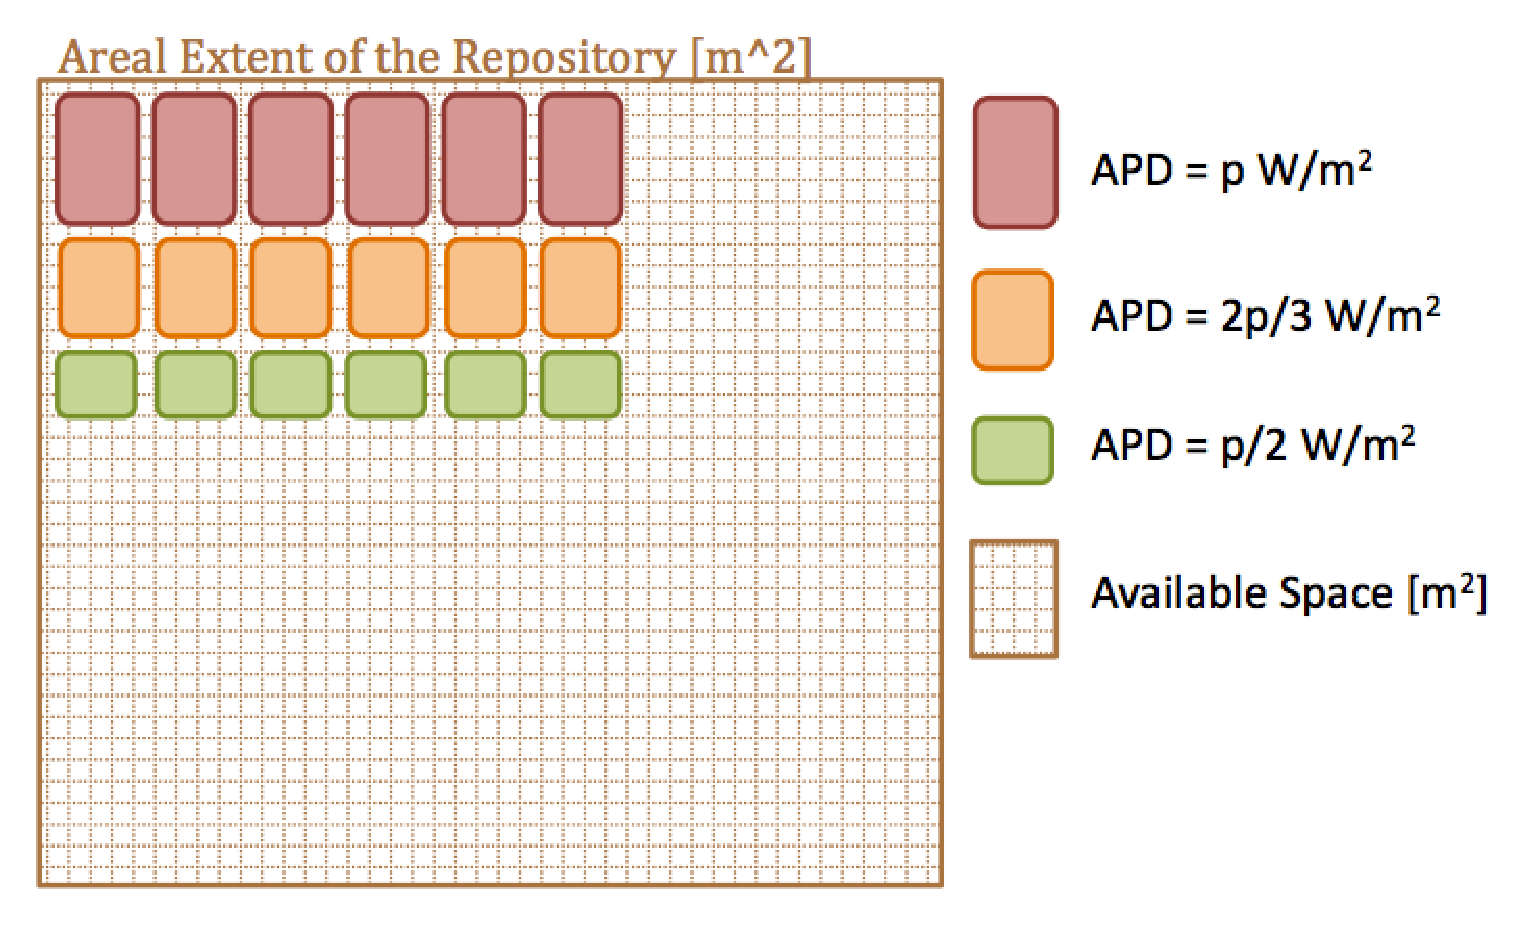
\includegraphics[width=0.7\textwidth]{APD.eps}
      \caption{The areal power density loading scheme pictured above is not 
      constrained by uniform spacing and takes advantage of denser spacing 
      made possible by cooler packages (green).  }
      \label{fig:apd}
      \end{center}
\end{figure}

In the areal power density loading schem, loading is subject to the constraints,
    \begin{align}
      P_{tot} &\le P_{max} \\
      APD_i &\le APD_{max}
      \intertext{where}
      P_{max} &= A\cdot APD_{max}\\ 
      P_{tot} &= \sum_{i=0}^{N}n_i P_i\\ 
      P_i &= \mbox{power of package i}\nonumber\\
      n_i &= \mbox{ith package}\nonumber\\
      N &= \mbox{number of packages}\nonumber\\
      APD_{max} &= \mbox{max areal power density}\nonumber
    \end{align}

\subsubsection{Peak Heat Approximation}

One conservative estimation could assume that $Q(t)$ is a constant heat flux, 
$Q_{max}$ equal to the peak of calculated waste form heat evolution, 
$max(Q(t))$. Assuming $Q(t) = Q_{max} \forall t$, it would be possible to 
directly refer to previously calculated repository evolution results 
based on constant heat and spacing. 

\begin{figure}[htb!]
  \begin{center}
    \def\svgwidth{.7\textwidth}
    \input{acceptance.eps_tex}
  \end{center}
  \caption{Above the empirically determined acceptance threshold for a certain 
  $K_{th}, \alpha_{th}$ combination, the arbitrary  waste stream is likely to be 
  acceptable. Below it, the waste stream is likely to be unacceptable. }
  \label{fig:acceptance}
\end{figure}

\subsubsection{Heat Integral Approximation}

Another approximation could develop the heat and spacing thresholds based on the 
integral of heat over time. Then, the time evolution of $Q(t)$ could be captured  
in the comparison. 

\begin{figure}[htb!]
  \begin{center}
    \def\svgwidth{.7\textwidth}
    \input{acceptanceInt.eps_tex}
  \end{center}
  \caption{Above the empirically determined acceptance threshold for a certain 
  $K_{th}, \alpha_{th}$ combination, the arbitrary  waste stream is likely to be 
  acceptable. Below it, the waste stream is likely to be unacceptable. }
  \label{fig:acceptanceInt}
\end{figure}

One method in the literature not dissimilar to this is the Specific Temperature 
Integral by Jun Li\cite{li_specific_2008}. 

A specific temperature integral may model the thermal source as linear along the
emplacement paths, analagously to the areal power density method.
However, a temperate integral takes account of heat transfer behavior in the
rock, includes the effects of myriad SNF compositions, and gives the thermal
integration over time for any specific location within the rock.  Man-Sung Yim
calls this the Specific Temperature Increase method\cite{li_specific_2008}.

In the same way that $Q(t)$, the heat flux from the waste streams, can be
expressed as the superposition of the linear heat flux contributions of all the
radionuclides in the waste, he temperature change
expressed as a superposition of the temperature change contributions due to  
each radionuclide. Each radionuclide contributes in proportion to its
decay heat generation and its weight fraction of the SNF. With information
about isotopic composition of the SNF, the specific temperature increase can
determine the maximum thermal capacity of the repository in terms of tonnes/m.
The length based accounting in $\frac{t}{m}$ is converted to
$\frac{t}{Repository}$ by multiplication with the total emplacement tunnel
length of the repository. 

\subsubsection{Effective Mean Decay Power}

Introduced by Radel, Wilson et. al., the Specific Temperature Change method uses 
a linear approximation to arrive at the thermal loading density limit.  

The mean decay constant of the radionuclide constituents in the waste form was 
compared to the thermal time constant in the rock. 

When the thermal time constant of the rock is much shorter than the waste form 
decay package, the change in package wall temperature can be described by 

\begin{align}
q(t_0)\rho_{limit}C'&=\Delta T_1
\label{fig:Tracyfig}
\intertext{where}
\rho_{limit} &= \frac{C_1}{Q_1}\nonumber\\
C' &= \mbox{ Thermal constant }[-]\nonumber\\
\Delta T &= \mbox{ Constant difference between }T_{lim}\mbox{ and }T_{amb}[^{\circ}C]\nonumber\\
T_{lim} &= \mbox{ Temperature limit }[^{\circ}C]\nonumber\\
T_{amb} &= \mbox{ Ambient rock temperature }[^{\circ}C]\nonumber
\end{align}

\subsubsection{Thermal Half-Life Approximation}

There is some notion of a thermal halflife in the literature. 



\subsection{Waste Stream Loading Density in Waste Forms}

Either the user inputs the waste form loading density or the repository must 
determine how best to load the waste forms with waste .

\subsection{Waste Package Loading Strategy in Repository}

Either the user inputs the tunnel spacing and waste package spacing, or the 
repository must determine how best to space the tunnels and packages.

\subsection{Solving for the Heat Evolution}

This model should be capable of calculating the temperature field through the 
repository over time for a certain waste package layout. 


\pagebreak
\bibliographystyle{ieeetr}
\bibliography{lecture}
\end{document}
